\section{\gls{fpga}}

A field-programmable gate array (\gls{fpga}) is a integrated circuit designed to be configured after the manufacturing. FPGAs can be used to test and debug implementations of hardware circuits and can be configured as hardware accelerators. In this project, we have use a Xilinx \gls{fpga} to simulate and test the design of a multi-core RISC-V. This section is dedicated to introduce the main characteristics of an \gls{fpga}, its architecture and an overview of the resources available on the \gls{fpga} board that we have used.

\subsection{FPGA Architecture}
An FPGA has a regular structure of logic cell or modules that are interconnected in a matrix form. The main components are:

\begin{itemize}
	\item \textbf{Configurable Logic Block (CLB):} it is the basic logic resource. It can implement logic functions throught a Look-up Table and contains flip-flops and multiplexers. 
	\item \textbf{I/O Blocks:} the Input/Output blocks are used to access the peripherals. 
	\item \textbf{Switch Matrix:} network of switches that is used interconnect CLBs and I/O blocks in a flexible way.
\end{itemize}

As it is shown in figure \ref{fig:fpga}, the components are distributed in a regular  form. The Bitstream is loaded to provide logical functions and interconnections of different blocks. 

\begin{figure}[h]
    \centering
    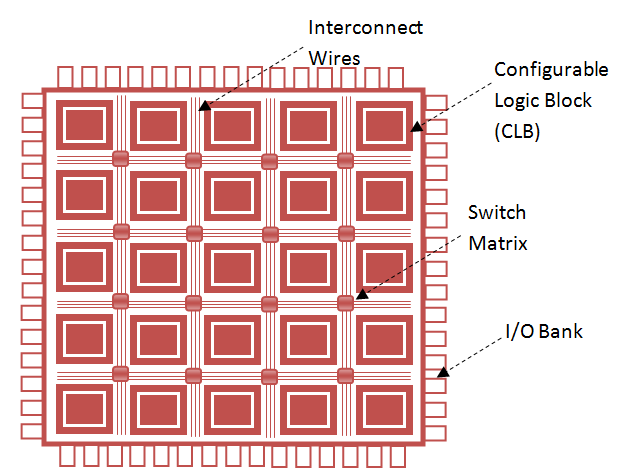
\includegraphics[width=0.8\textwidth]{../presentation/images/FPGA-Architecture.png}
    \caption{Schematic representation of an FPGA chip} Reproduced from \cite{FPGA}.
    \label{fig:fpga}
\end{figure}

\subsection{Xilinx Spartan 7 SP701} \label{sec:fpga}
\gls{sp7} is the model of the board where we will run a RISC-V core. It is built for designs requiring sensor fusion such as industrial networking, embedded vision, and automotive applications. This product is uncommon material since the specialized target of users and the high cost. At this point, it is important to distinguish between the board and the \gls{fpga} chip. The XC7S100 is the Spartan Series 7 chips which is assembled in the board. The resources available are \cite{xilinxsp}:  

\begin{itemize}
	\item \textbf{\gls{fpga} chip:}
	\begin{itemize}
		\item \textbf{102400 Logic elements (LE)}: smallest units of logic (8 bit Look-up Table). LEs  provide advanced features with efficient logic like LUT
	   	\item \textbf{16000 Adaptive Logic Module (ALM)}: more complex boolean using up to 16 bit Look-up Tables functions with/without registers
	    	\item 400 I/O operations per second %Input output operations per second 
	\end{itemize}
	\item \textbf{Board  Resources:}
	\begin{itemize}
		\item \textbf{Memory:} DDR3L 4Gb (256M x 16)
		\item \textbf{5 pushbuttons}
		\item \textbf{16 DIP switches}
		\item \textbf{8 LEDs}
		\item \textbf{HDMI Video Output}
		\item \textbf{2 RJ-45}
		
	\end{itemize}
\end{itemize}

These are the resources where we will fit out RISC-V core. It is a limiting aspect that is going to be critical in the election of the core. Modifications at the core structure can be considered in order to fit the harware in the FPGA. 




